\chapter{Preliminaries}
\label{chap:preliminaries}

\section{Transformer-Based Vision-Language Models}

\subsection{Transformer Basics}

Modern vision-language models are built on the Transformer architecture
\cite{vaswani2023attentionneed}. For an input sequence, self-attention maps query,
key and value matrices \(\mathbf{Q}\), \(\mathbf{K}\) and \(\mathbf{V}\) to
\begin{equation}
\mathrm{Attention}(\mathbf{Q},\mathbf{K},\mathbf{V})
=
\mathrm{softmax}\!\left(\frac{\mathbf{Q}\mathbf{K}^{\top}}{\sqrt{d_k}}\right)\mathbf{V},
\end{equation}
where \(d_k\) is the key dimension. Multi-head attention runs this operation
in parallel across several learned subspaces, then applies a feed-forward
network and residual normalization.

For language modeling, the Transformer produces a sequence of hidden states and
next-token logits. In this thesis, the student and teacher interact through
their output logits because the distillation method operates at the
token-distribution level \cite{vaswani2023attentionneed,hinton2015distillingknowledgeneuralnetwork}.

\begin{figure}[tp]
    \centering
    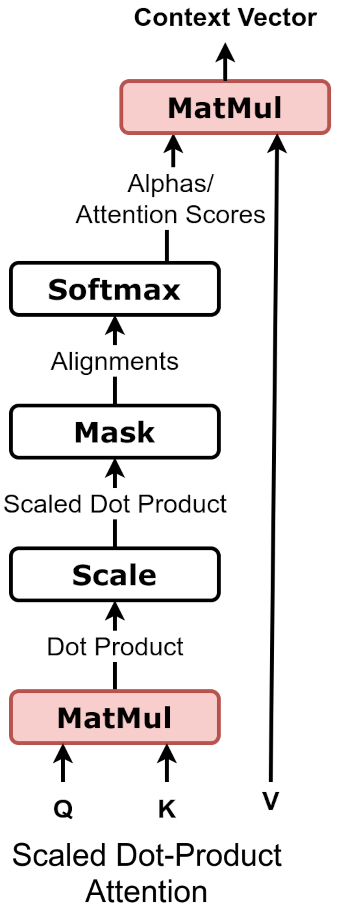
\includegraphics[height=0.20\textheight,keepaspectratio]{figures/transformer_attention_block_wikimedia.png}
    \caption{Transformer attention block structure \cite{wikimedia_transformer_attention_block_image,vaswani2023attentionneed}. The figure isolates the attention and feed-forward block that is later reused in both language and vision stacks.}
    \label{fig:prelim-transformer-attention}
\end{figure}

\subsection{Vision Encoder and Multimodal Fusion}

On the visual side, many multimodal systems use a Vision Transformer (ViT)
\cite{dosovitskiy2021imageworth16x16words}, which converts an image into a sequence
of patch embeddings and processes them with Transformer blocks. A connector
module then fuses these visual tokens with text, using cross-attention, a Q-Former,
or a learned projector
\cite{alayrac2022flamingovisuallanguagemodel,li2023blip2bootstrappinglanguageimagepretraining,liu2023visualinstructiontuning}.

This thesis focuses on compact generative VLMs in the same general family as
SmolVLM and related projector-based models. Conceptually, we can write such a model as
\begin{equation}
\mathbf{z} = f_{\theta}(x),
\end{equation}
where \(x\) is a multimodal input and \(\mathbf{z}\) denotes the output logits
used for autoregressive answer generation.

\begin{figure}[tp]
    \centering
    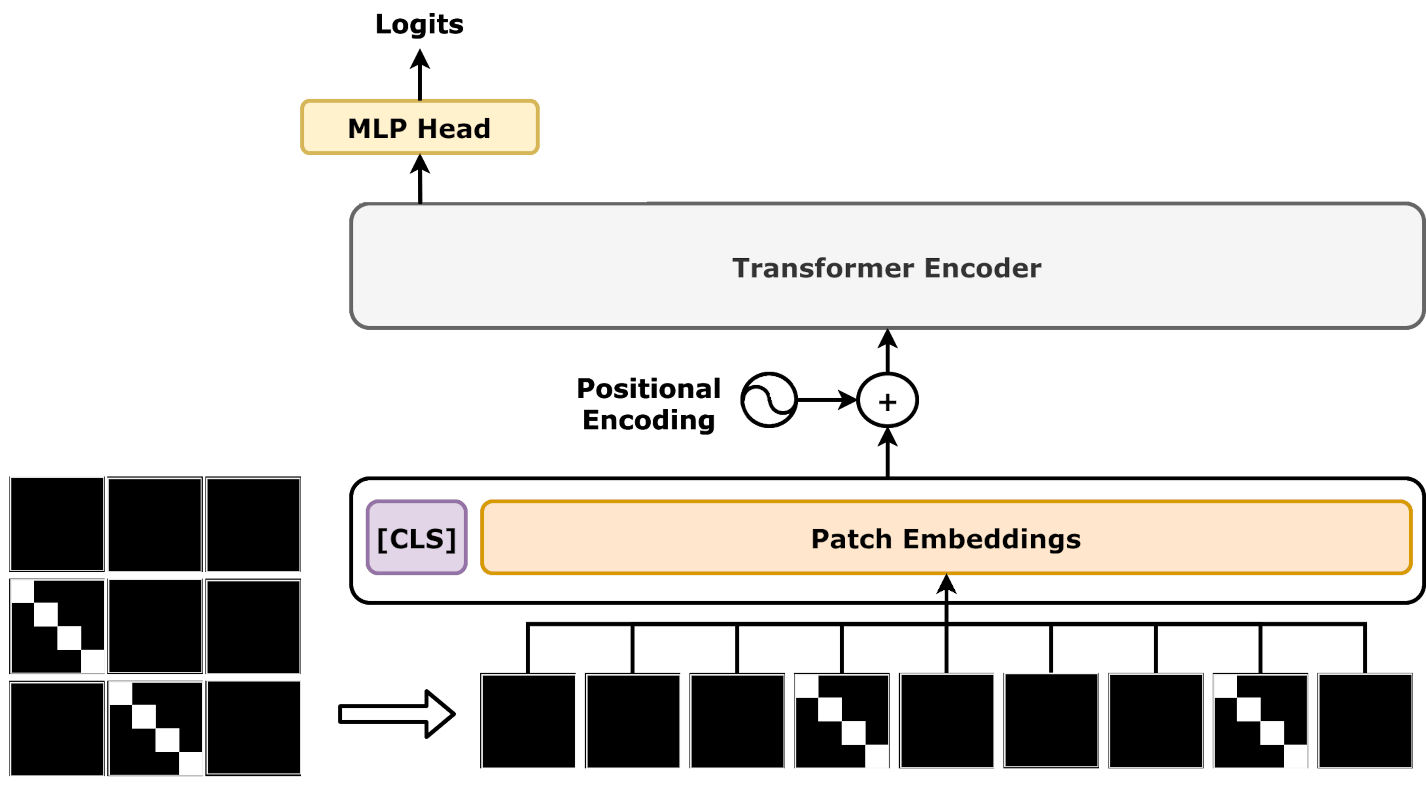
\includegraphics[width=0.68\linewidth]{figures/vit_wikimedia.png}
    \caption{Vision Transformer pipeline with patch embedding and Transformer encoder blocks \cite{wikimedia_vision_transformer_image,dosovitskiy2021imageworth16x16words}. It shows how an image becomes a token sequence before multimodal fusion.}
    \label{fig:prelim-vit}
\end{figure}

Figures~\ref{fig:prelim-transformer-attention} and \ref{fig:prelim-vit} give
the basic Transformer and ViT blocks that later multimodal systems build on.

\begin{figure}[tp]
    \centering
    \begin{subfigure}[t]{0.48\linewidth}
        \centering
        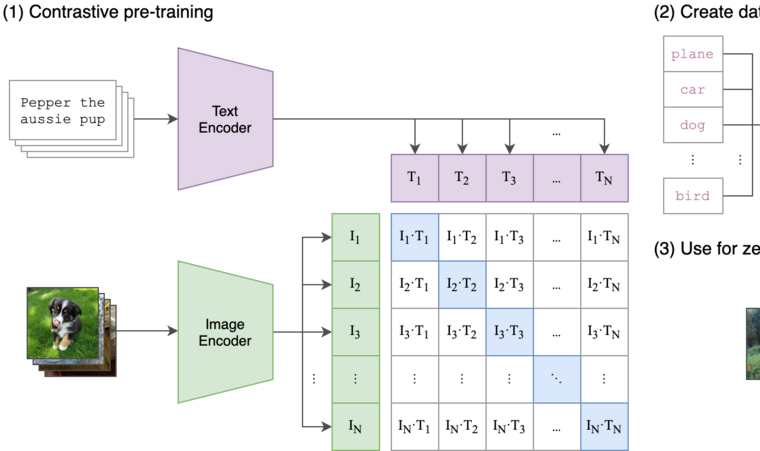
\includegraphics[width=\linewidth]{figures/clip_architecture_family.png}
        \caption{CLIP-style dual encoder \cite{radford2021learningtransferablevisualmodels}.}
    \end{subfigure}
    \hfill
    \begin{subfigure}[t]{0.48\linewidth}
        \centering
        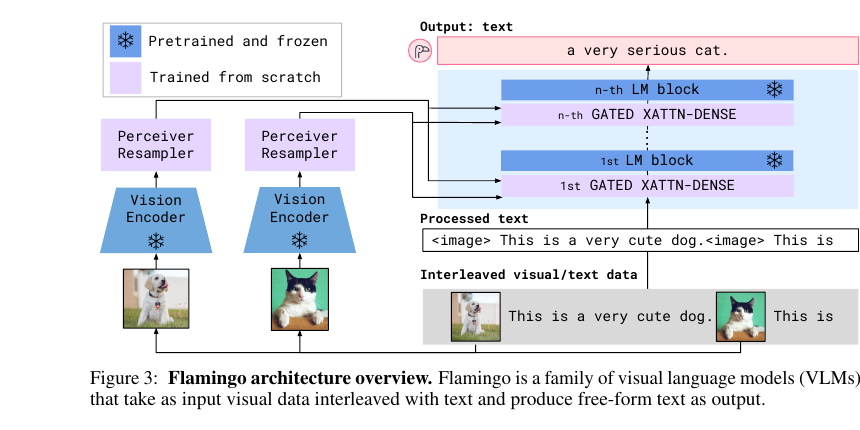
\includegraphics[width=\linewidth]{figures/flamingo_architecture_family.png}
        \caption{Flamingo cross-attention design \cite{alayrac2022flamingovisuallanguagemodel}.}
    \end{subfigure}

    \vspace{0.6em}

    \begin{subfigure}[t]{0.48\linewidth}
        \centering
        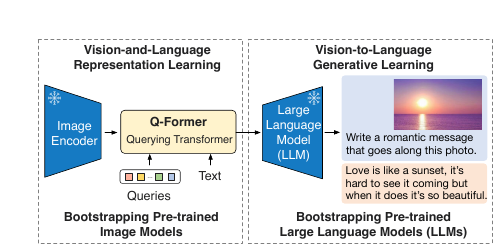
\includegraphics[width=\linewidth]{figures/blip2_architecture_family.png}
        \caption{BLIP-2 with Q-Former \cite{li2023blip2bootstrappinglanguageimagepretraining}.}
    \end{subfigure}
    \hfill
    \begin{subfigure}[t]{0.48\linewidth}
        \centering
        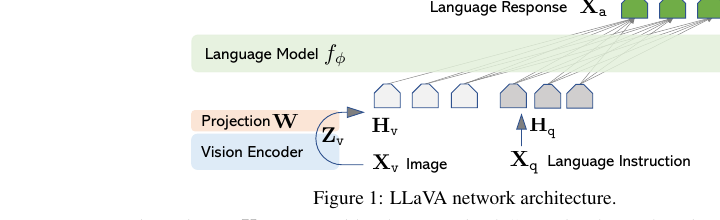
\includegraphics[width=\linewidth]{figures/llava_architecture_family.png}
        \caption{LLaVA projector-based design \cite{liu2023visualinstructiontuning}.}
    \end{subfigure}
    \caption{Representative architecture families of modern vision-language models. Together they show the main fusion choices used in practice: dual encoders, cross-attention, query bottlenecks and projector-based coupling to a language model.}
    \label{fig:prelim-vlm-families}
\end{figure}

\subsection{Text-Rich Multimodal Understanding}

The tasks considered in this thesis, namely TextVQA, DocVQA and ChartQA, require
the model to read text in images, understand the question and perform basic
reasoning over visual and textual evidence
\cite{singh2019vqamodelsread,mathew2021docvqadatasetvqadocument,masry2022chartqabenchmarkquestionanswering}.
This setting differs from generic image captioning because success depends strongly
on optical character recognition (OCR)-sensitive recognition and token-level answer generation.

\begin{figure}[tp]
    \centering
    \begin{subfigure}[t]{0.31\linewidth}
        \centering
        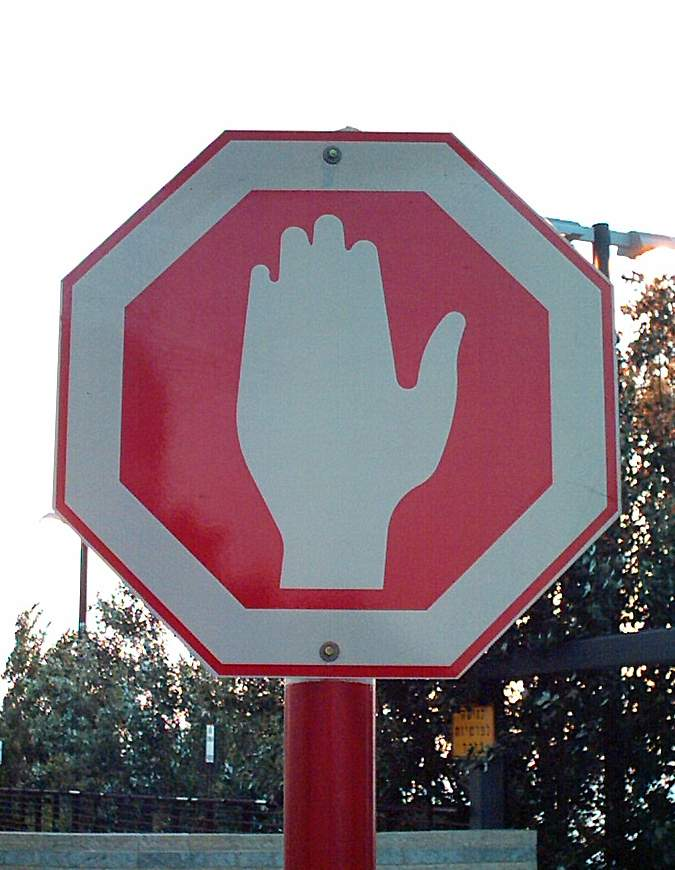
\includegraphics[width=\linewidth,height=0.18\textheight,keepaspectratio]{figures/textvqa_sample_stop_sign.jpg}
        \caption{TextVQA}
    \end{subfigure}
    \hfill
    \begin{subfigure}[t]{0.31\linewidth}
        \centering
        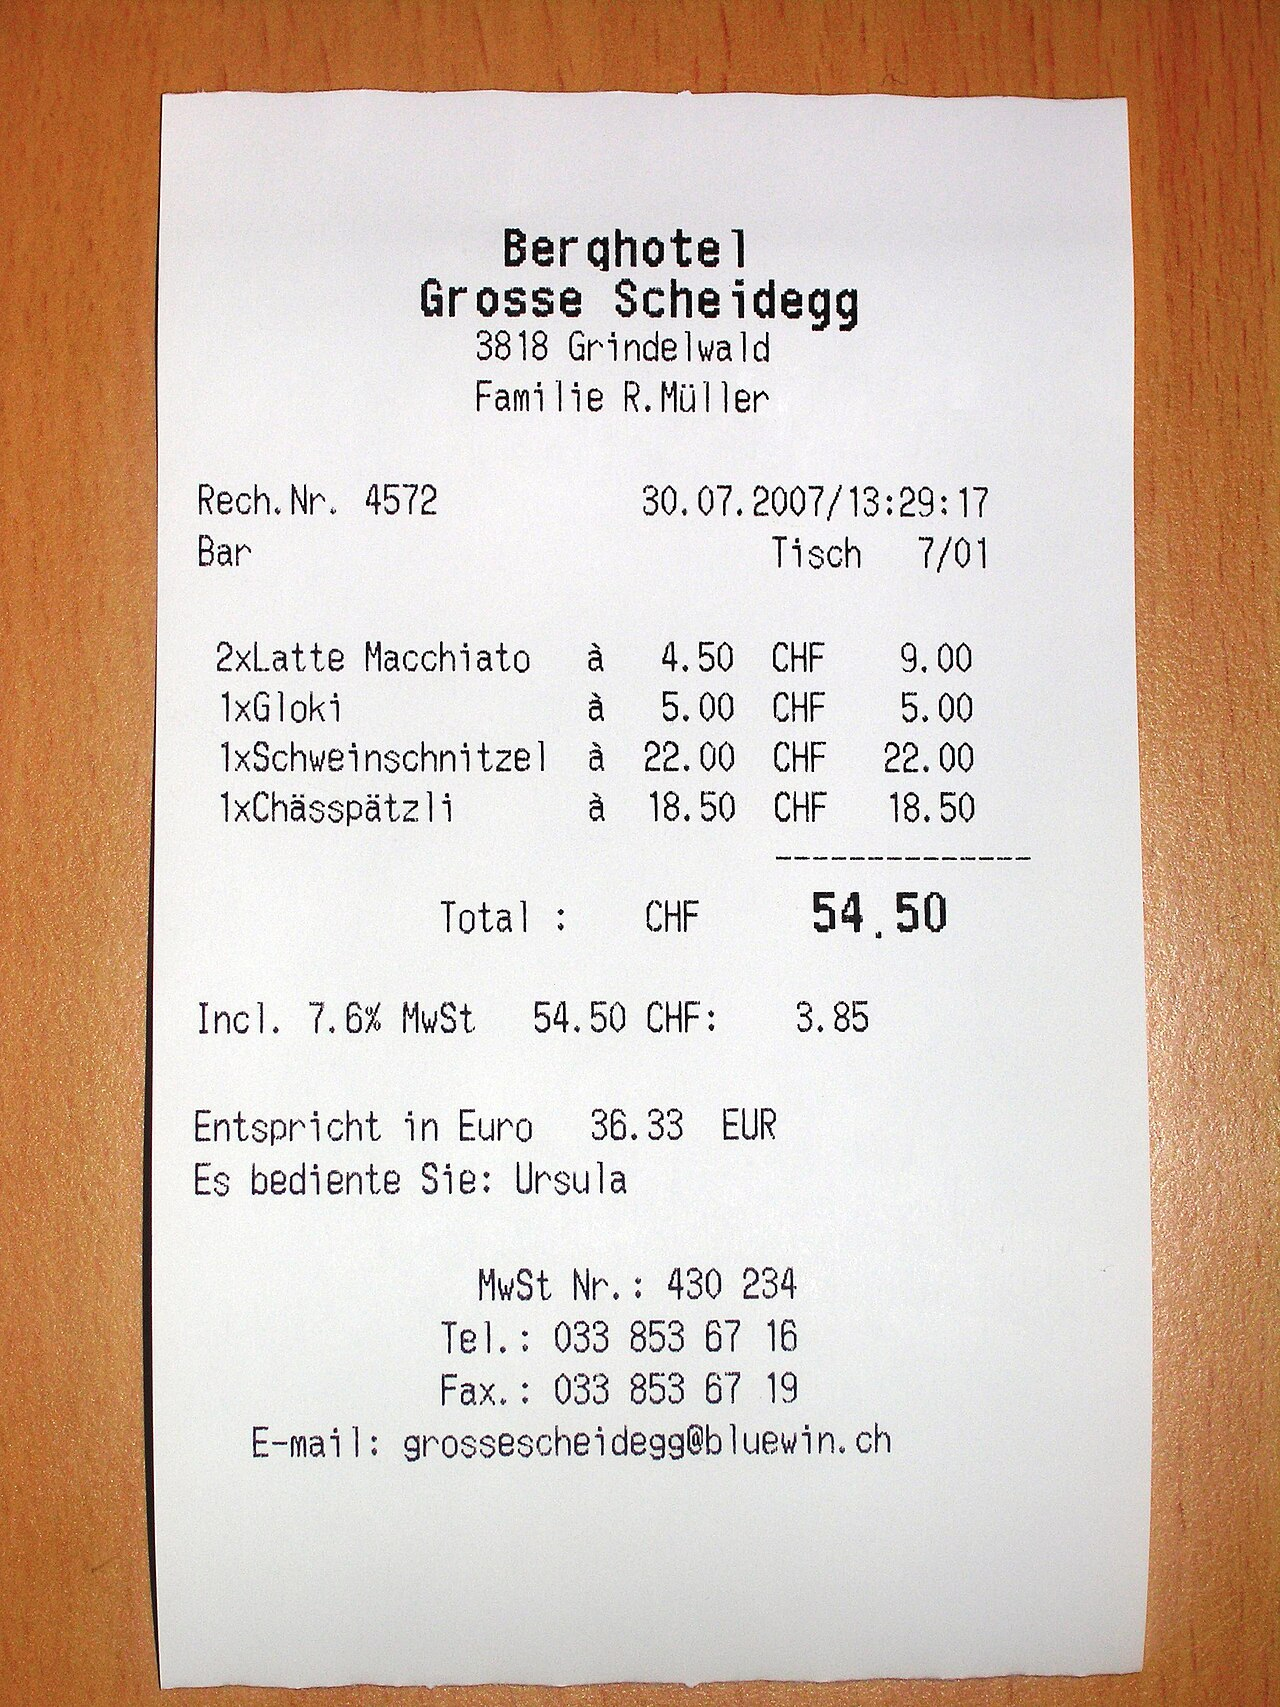
\includegraphics[width=\linewidth,height=0.18\textheight,keepaspectratio]{figures/docvqa_sample_receipt.jpg}
        \caption{DocVQA}
    \end{subfigure}
    \hfill
    \begin{subfigure}[t]{0.31\linewidth}
        \centering
        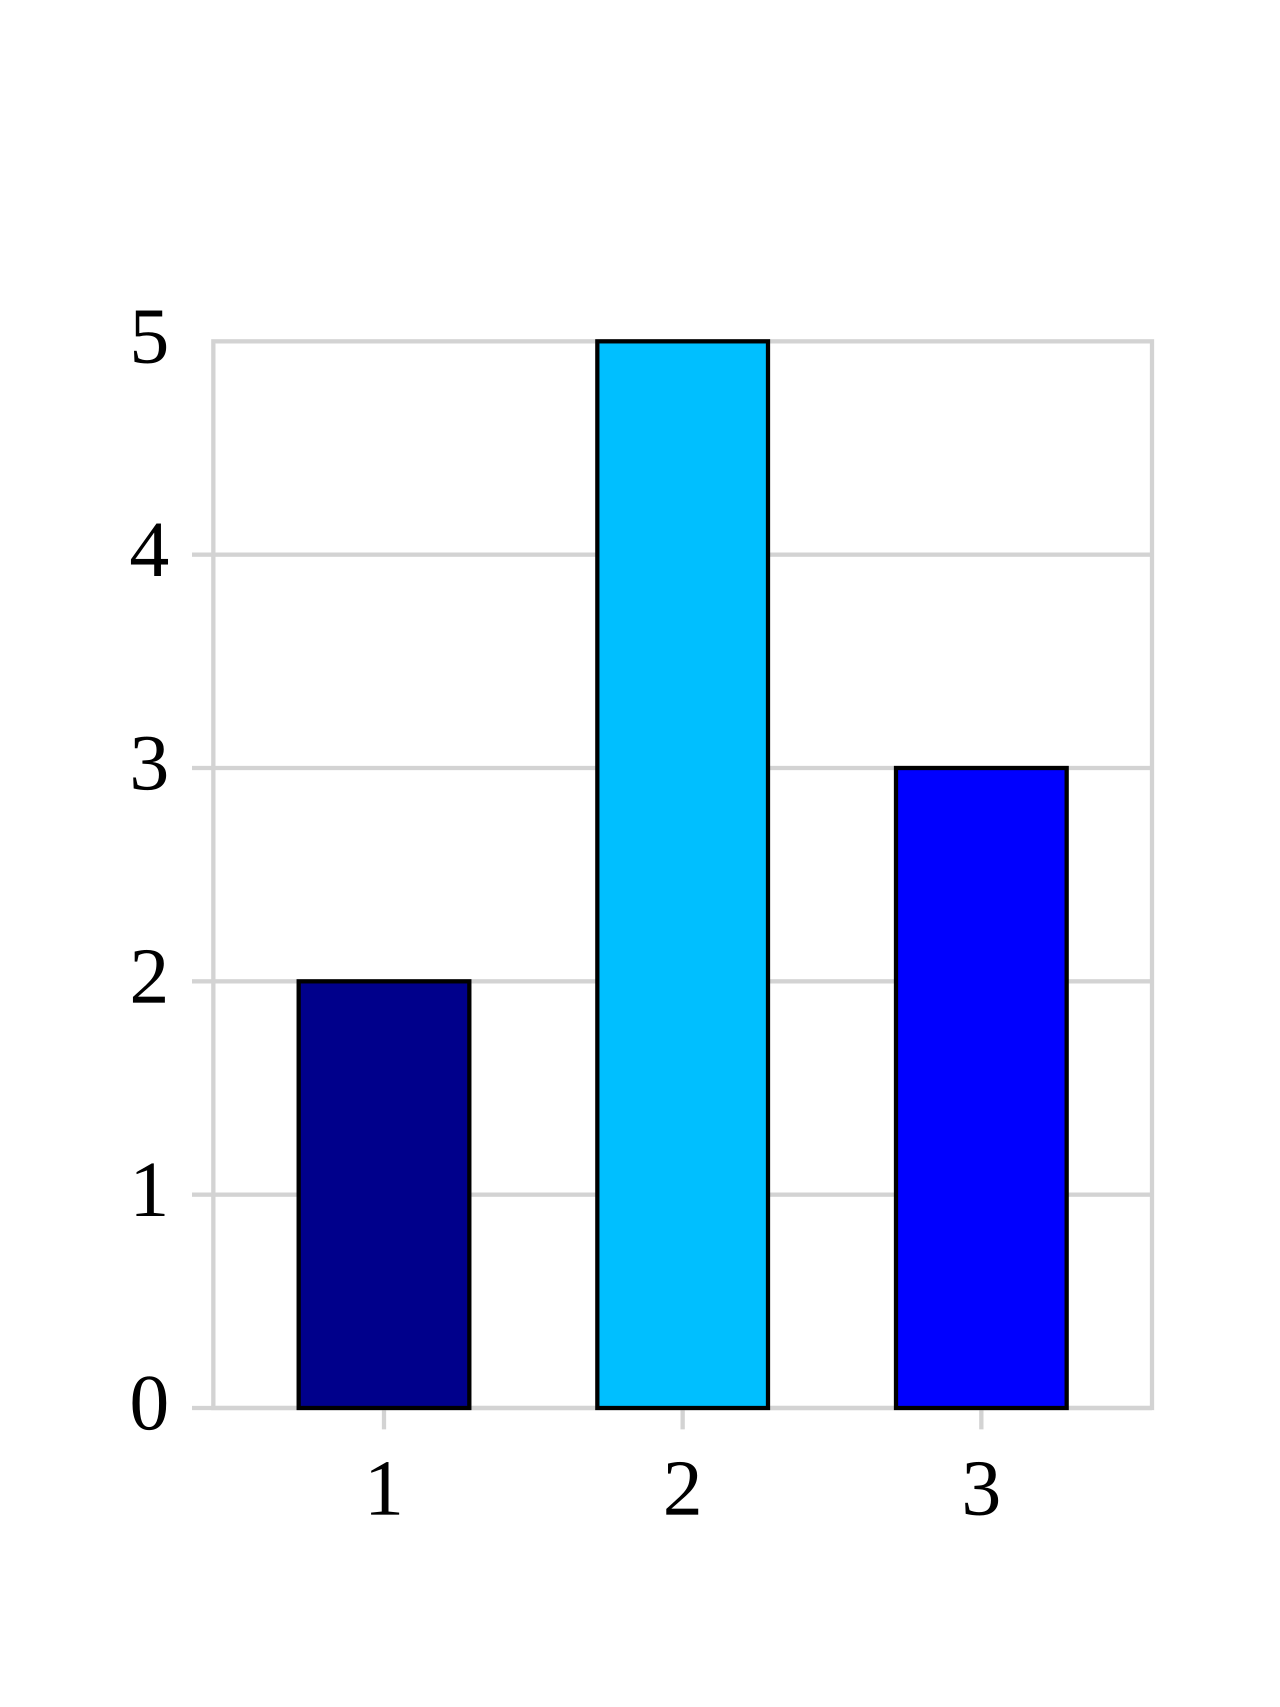
\includegraphics[width=\linewidth,height=0.18\textheight,keepaspectratio]{figures/chartqa_sample_bar_chart.png}
        \caption{ChartQA}
    \end{subfigure}
    \caption{Representative inputs from the text-rich multimodal benchmarks considered in this thesis \cite{singh2019vqamodelsread,mathew2021docvqadatasetvqadocument,masry2022chartqabenchmarkquestionanswering}. The three examples show why text reading, layout parsing and visual reasoning all matter in this benchmark suite.}
    \label{fig:prelim-benchmark-examples}
\end{figure}

Figure~\ref{fig:prelim-vlm-families} summarizes the main architecture families,
while Figure~\ref{fig:prelim-benchmark-examples} shows the text-rich inputs
used in this thesis.

\section{Knowledge Distillation}

\subsection{Teacher-Student Learning}

Knowledge distillation transfers information from a stronger teacher model to a
smaller student model \cite{hinton2015distillingknowledgeneuralnetwork,xu2024surveyknowledgedistillationlarge}.
Let \(\mathcal{L}_{CE}\) denote the supervised cross-entropy loss of the student.
A generic distillation objective takes the form
\begin{equation}
\mathcal{L}
=
\lambda_{CE}\mathcal{L}_{CE}
+
\lambda_{KD}\mathcal{L}_{KD},
\end{equation}
where \(\mathcal{L}_{KD}\) is a teacher-guided loss. In later chapters, GRACE
instantiates this template with a routed trie-Wasserstein term plus small router
regularizers.

In token-level distillation, the teacher and student are compared on their output
logits, not only on hard labels. This allows the student to learn richer
distributional structure, often called \emph{dark knowledge} \cite{hinton2015distillingknowledgeneuralnetwork}.

\begin{figure}[tp]
    \centering
    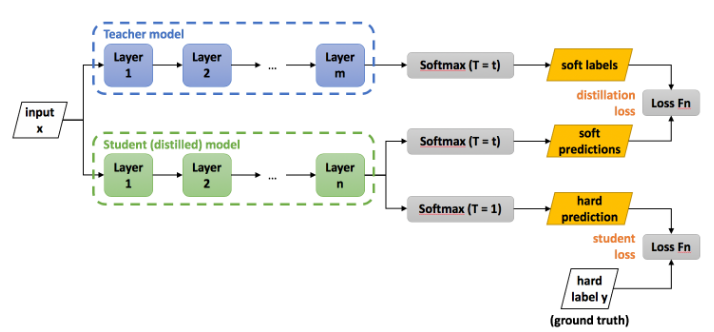
\includegraphics[width=0.78\linewidth]{figures/knowledge_distillation_example.png}
    \caption{Generic teacher-student knowledge distillation setup with hard labels and soft targets \cite{wikimedia_knowledge_distillation_example,hinton2015distillingknowledgeneuralnetwork}. It provides the basic supervision pattern before GRACE adds heterogeneous teachers and routing.}
    \label{fig:prelim-kd-overview}
\end{figure}

Figure~\ref{fig:prelim-kd-overview} provides the generic teacher-student
template before Chapter~\ref{chap:proposed-method} specializes it to GRACE.

\subsection{Temperature-Scaled Output Distributions}

Let \(\mathbf{z}_s\) and \(\mathbf{z}_t\) denote student and teacher logits.
With temperatures \(\tau_s\) and \(\tau_t\), the corresponding distributions are
\begin{equation}
\mathbf{p}_s = \mathrm{softmax}\!\left(\frac{\mathbf{z}_s}{\tau_s}\right),
\qquad
\mathbf{p}_t = \mathrm{softmax}\!\left(\frac{\mathbf{z}_t}{\tau_t}\right).
\end{equation}

Many classical KD methods compare \(\mathbf{p}_s\) and \(\mathbf{p}_t\) using
divergences such as forward KL or Jensen-Shannon divergence. However, such
approaches usually assume that teacher and student share the same vocabulary
\cite{hinton2015distillingknowledgeneuralnetwork,lin1991jensen,boizard2024towardscrosstokenizerdistillation}.

\section{Cross-Tokenizer Distillation Background}

\subsection{Motivation}

In this thesis, the teacher pool may contain different VLM families with
different tokenizers and vocabulary sizes. A KD loss that assumes a shared
output space is therefore too restrictive. Universal Logit Distillation (ULD)
is one important prior remedy because it avoids direct token-ID matching
\cite{boizard2024towardscrosstokenizerdistillation}. Chapter~\ref{chap:proposed-method}
later replaces the ranked-mass surrogate with a trie-Wasserstein variant that
keeps the same cross-tokenizer goal but uses a tree-structured transport view.

\begin{figure}[tp]
    \centering
    \includegraphics[width=0.58\linewidth]{figures/uld_vocab_overlap.png}
    \caption{Vocabulary-overlap ratios between teacher and student tokenizers from the ULD paper \cite{boizard2024towardscrosstokenizerdistillation}. The overlap is far from complete, which makes direct token-ID KD unreliable across model families.}
    \label{fig:prelim-uld-overlap}
\end{figure}

Figure~\ref{fig:prelim-uld-overlap} makes the mismatch explicit: even strong
teacher-student pairs can share only part of their vocabularies.

\subsection{ULD as a Prior Baseline}

Given student logits \(\mathbf{z}_s \in \mathbb{R}^{V_s}\) and teacher logits
\(\mathbf{z}_t \in \mathbb{R}^{V_t}\), we first compute their temperature-scaled
probability distributions \(\mathbf{p}_s\) and \(\mathbf{p}_t\). We then sort both
vectors in descending order, pad the smaller vocabulary with zeros and compare
the sorted masses with an \(L_1\) distance:
\begin{equation}
\mathcal{L}_{ULD}(\mathbf{z}_s,\mathbf{z}_t)
=
\left\|
\pi(\mathbf{p}_s)-\pi(\mathbf{p}_t)
\right\|_1,
\end{equation}
where \(\pi(\cdot)\) denotes sorting in descending order after zero-padding.

The key advantage of ULD is that it compares distributions by ranked
probability mass instead of token identity. This makes it directly
applicable to cross-tokenizer teacher-student distillation
\cite{boizard2024towardscrosstokenizerdistillation}. In the later experiments,
ULD is treated as a cross-tokenizer baseline, not the final method.

\begin{figure}[tp]
    \centering
    \includegraphics[width=0.88\linewidth]{figures/uld_pipeline.png}
    \caption{ULD pipeline from the original paper \cite{boizard2024towardscrosstokenizerdistillation}. Teacher and student probabilities are sorted and zero-padded before the ranked masses are compared, which removes the need for direct vocabulary alignment.}
    \label{fig:prelim-uld-pipeline}
\end{figure}

\subsection{Optimal Transport and Tree-Structured Mass Matching}

Optimal transport compares two probability measures by the minimum cost required
to move mass from one distribution to the other
\cite{peyre2019computationaloptimaltransport}. For discrete source weights
\(\mathbf{a}\), target weights \(\mathbf{b}\) and transport cost matrix
\(\mathbf{C}\), the corresponding optimization problem can be written as
\begin{equation}
W(\mathbf{a},\mathbf{b})
=
\min_{\mathbf{P}\in\mathcal{U}(\mathbf{a},\mathbf{b})}
\langle \mathbf{P}, \mathbf{C} \rangle,
\qquad
\mathcal{U}(\mathbf{a},\mathbf{b})
=
\left\{
\mathbf{P}\ge 0 \mid
\mathbf{P}\mathbf{1}=\mathbf{a},\
\mathbf{P}^{\top}\mathbf{1}=\mathbf{b}
\right\}.
\end{equation}
Here, \(\mathbf{P}\) is a transport plan that specifies how much mass is moved
from each source bin to each target bin.

\begin{figure}[tp]
    \centering
    \includegraphics[width=0.78\linewidth]{figures/continuous_optimal_transport_wikimedia.png}
    \caption{Continuous displacement view of optimal transport \cite{wikimedia_continuous_optimal_transport_image,peyre2019computationaloptimaltransport}. The figure emphasizes the geometric side of OT: mass is moved through space with a transport map, not compared by fixed bin identity alone.}
    \label{fig:prelim-continuous-ot}
\end{figure}

Figure~\ref{fig:prelim-continuous-ot} gives the continuous geometric view of
OT. The same idea appears in the discrete case through a transport plan
\(\mathbf{P}\), and later in the tree case through edgewise subtree mass.

This viewpoint also motivates tree-structured transport. When teacher and
student have different vocabularies, matching probabilities by token index is
not meaningful. What matters instead is how probability mass sits on a
shared structure \cite{boizard2024towardscrosstokenizerdistillation,peyre2019computationaloptimaltransport}.

Tree-Wasserstein distances make that idea explicit by placing probability mass
on a tree metric and summing weighted subtree imbalances
\cite{takezawa2021supervisedtreewasserstein,peyre2019computationaloptimaltransport}.
For a rooted tree \(T=(V,E)\) with edge weights \(w(e)\), one convenient form is
\begin{equation}
W_T(\mu,\nu)
=
\sum_{e\in E}
w(e)\,
\left|
\mu\!\left(\Gamma(e)\right)-\nu\!\left(\Gamma(e)\right)
\right|,
\end{equation}
where \(\Gamma(e)\) denotes the subtree below edge \(e\). The key point is that,
on a tree metric, transport decomposes into edgewise subtree-mass imbalance
instead of a dense source-target coupling
\cite{takezawa2021supervisedtreewasserstein,leyamadafukumizucuturi2019treesliced}.
This is computationally attractive because the comparison follows the tree
structure directly and it is conceptually natural when tokens share prefixes or
other hierarchical relations.

\begin{figure}[tp]
    \centering
    \includegraphics[width=0.78\linewidth]{figures/tree_wasserstein_stw_paper.png}
    \caption{Example tree metrics from Quadtree, tree-sliced Wasserstein (TSW) and supervised tree-Wasserstein (STW) on a synthetic dataset \cite{takezawa2021supervisedtreewasserstein}. The comparison is not a VLM result, but it makes the tree-transport idea explicit: mass is organized along branches of a hierarchy instead of through one dense transport matrix.}
    \label{fig:prelim-tree-ot}
\end{figure}

Tree-sliced OT extends the same idea by averaging Wasserstein distances over
tree metrics and shows that tree metrics preserve the geometric view of OT while
admitting fast closed-form computations
\cite{leyamadafukumizucuturi2019treesliced}. In this thesis, the relevant tree
is not an abstract hierarchy but the shared UTF-8 byte trie induced by teacher
and student decoded single-token strings.

That perspective is closer to the trie-Wasserstein loss used later in
Chapter~\ref{chap:proposed-method}: the method maps tokens to paths on a shared byte
trie and compares mass on edges instead of token index.

\begin{figure}[tp]
    \centering
    \includegraphics[height=0.26\textheight,keepaspectratio]{figures/optimal_transport_matrix_wikimedia.png}
    \caption{Discrete transport plan matrix in optimal transport, showing how source and target marginals are coupled by a transport matrix \cite{wikimedia_optimal_transport_matrix_image,peyre2019computationaloptimaltransport}. The key idea is geometric: mass is compared by how it can be rearranged, not by fixed token identity.}
    \label{fig:prelim-optimal-transport}
\end{figure}

Figures~\ref{fig:prelim-continuous-ot}, \ref{fig:prelim-optimal-transport}
and \ref{fig:prelim-tree-ot} now cover the three views used later in the
thesis: geometric mass movement, discrete transport plans and tree-structured
mass matching. Chapter~\ref{chap:proposed-method} instantiates the third view
with a shared byte trie and a sparse tree-Wasserstein loss.

\subsection{Answer-Token Distillation}

For multimodal question answering, distillation should focus on answer tokens, not prompt tokens \cite{liu2023visualinstructiontuning}.

In our implementation, the code computes KD only on supervised answer positions after masking ignored tokens, optionally removing EOS and truncating student and teacher answer spans to a common length.

In Chapter~\ref{chap:proposed-method}, these sets are denoted by
\(\Omega_b^{CE}\) for CE and \(\Omega_{b,i}^{KD}\) for teacher-specific KD.

This gives a token-aligned distillation signal while remaining compatible with different tokenizers.

\section{Multi-Teacher Distillation}

\subsection{Per-Teacher KD Loss}

Let \(\mathcal{T}=\{T_1,\ldots,T_N\}\) be a pool of frozen teachers. For sample
\(b\), teacher \(T_i\) produces a per-teacher distillation loss
\(\mathcal{L}_{KD}^{(b,i)}\). In principle, one could average these losses uniformly,
\begin{equation}
\mathcal{L}_{KD}^{(b)}
=
\frac{1}{N}\sum_{i=1}^{N}\mathcal{L}_{KD}^{(b,i)},
\end{equation}
but this assumes every teacher is equally useful for every sample.

In practice, different teachers may provide conflicting guidance. Some teachers
may help the supervised objective on a given sample, while others may push the
student in a different direction \cite{zhu2021studentcustomized}. This motivates
a selective routing mechanism that decides, for each sample, which teachers
should be active.

\subsection{Learned Routing and Load Balancing}

Recent sparse expert models route each sample or token through only a subset of available experts. This improves efficiency and allows specialized computation \cite{shazeer2017outrageouslylargeneuralnetworks,fedus2022switchtransformersscalingtrillion,deepseekai2024deepseekv2strongeconomicalefficient}.

The same high-level idea is useful in multi-teacher distillation. Instead of averaging all teachers equally, a learned router can propose teacher weights from student-side features \cite{yuan2020reinforcedmultiteacherselection,zhang2023adaptivemultiteachermetalearning,yu2024selectdistill}.

Let \(\mathbf{h}^{(b)}\) denote a pooled student representation for sample \(b\).
A router network \(G(\cdot)\) produces gate logits
\begin{equation}
\mathbf{r}^{(b)} = G(\mathbf{h}^{(b)}),
\qquad
\tilde{\mathbf{r}}^{(b)} = \text{AdjustedScores}\!\left(\mathbf{r}^{(b)}\right),
\qquad
\mathbf{p}^{(b)} = \mathrm{softmax}\!\left(\tilde{\mathbf{r}}^{(b)}\right),
\end{equation}
where \(p_i^{(b)}\) is the initial routing weight for teacher \(T_i\). In the
current implementation, \(\tilde{\mathbf{r}}^{(b)}\) includes expert bias,
optional training noise and router-temperature scaling before softmax.

In sparse routing, these weights are typically refined by additional constraints:
\begin{enumerate}
\item \textbf{Top-\(k\) routing}, which keeps only the highest-scoring teachers.
\item \textbf{Capacity constraints}, which prevent one teacher from receiving too many assignments.
\item \textbf{Load balancing}, which discourages routing collapse onto a small subset of teachers.
\end{enumerate}

Following the general MoE literature, one can summarize the balancing signal by a
soft load \(\bar{p}_i\) and a hard assignment load \(\bar{q}_i\) after sparse
routing, capacity control and fallback and define an
auxiliary balancing objective of the form
\begin{equation}
\mathcal{L}_{bal}
=
N\sum_{i=1}^{N}\bar{p}_i \bar{q}_i.
\end{equation}
This auxiliary term does not replace the KD objective; instead, it regularizes
the router so that different teachers remain usable during training.

In \methodname, the code implements the router as a small student-conditioned MLP gate on
top of pooled student hidden states. It then applies softmax weights,
top-\(k\) sparsification and capacity filtering, with a short dense warmup
before sparse routing starts. The full framework also supports optional
balancing, entropy regularization and expert-bias updates.

When enabled, the expert bias term nudges the router toward under-used teachers
in subsequent batches.

This makes the routing stage closer to sparse-expert training than to a static teacher average \cite{shazeer2017outrageouslylargeneuralnetworks,fedus2022switchtransformersscalingtrillion,zhou2022mixtureofexpertswithexpertchoice}.

\begin{figure}[tp]
    \centering
    \includegraphics[width=0.80\linewidth]{figures/switch_capacity_routing_jmlr_clean2.png}
    \caption[Sparse routing with expert capacity constraints.]{Illustration of sparse routing with expert capacity constraints, adapted from Switch Transformers \cite{fedus2022switchtransformersscalingtrillion}. Capacity factors control how many routed samples each expert can accept before overflow, which is directly analogous to the capacity-aware teacher routing used in \methodname.}
    \label{fig:prelim-switch-routing}
\end{figure}

The next figure adds the specialization view. Sparse routing does not only save
compute, it also lets different experts focus on different inputs.

\begin{figure}[tp]
    \centering
    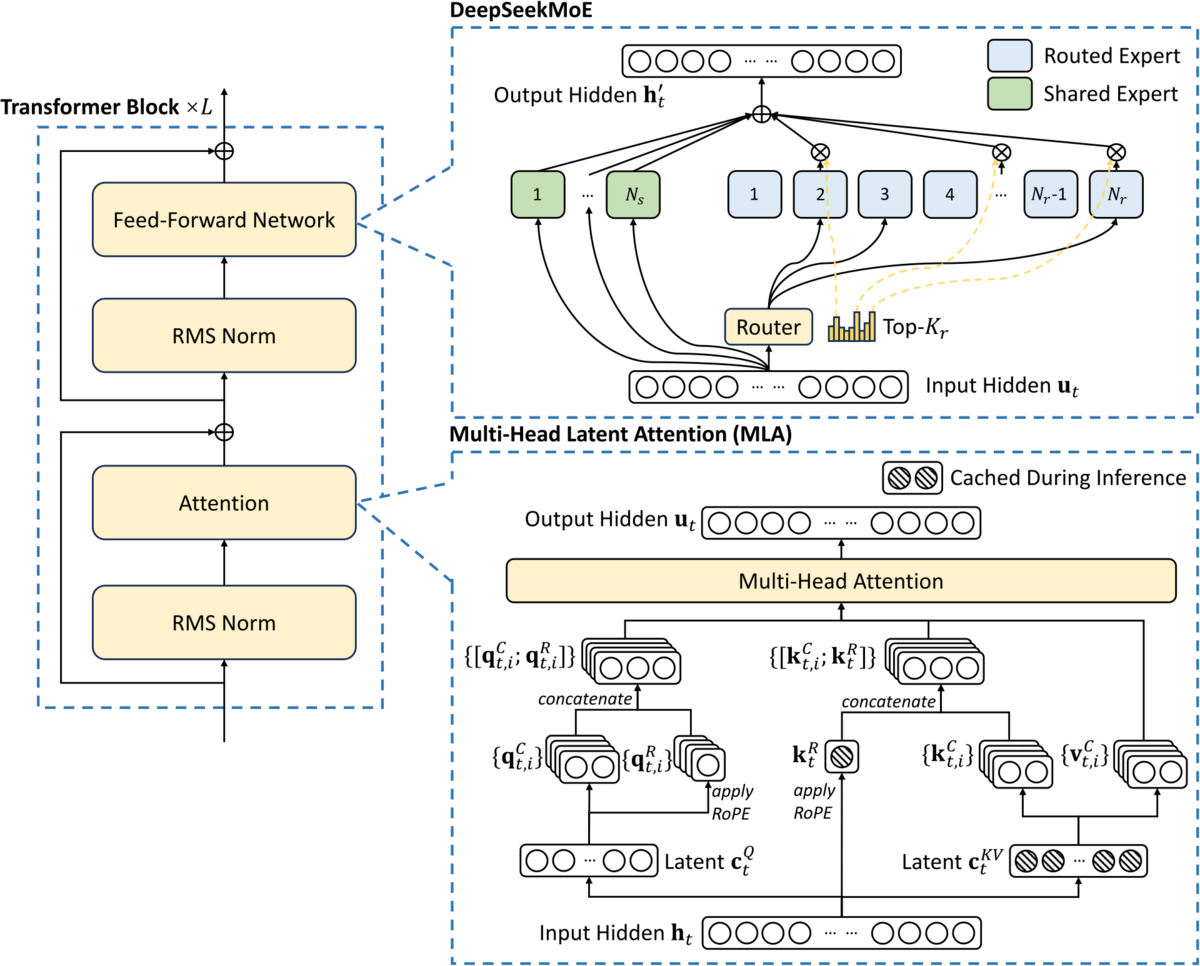
\includegraphics[width=0.78\linewidth]{figures/deepseek_moe_wikimedia.png}
    \caption[Sparse routing and expert specialization in MoE.]{Example of sparse routing and expert specialization in a mixture-of-experts architecture \cite{wikimedia_deepseek_moe_mla_image,deepseekai2024deepseekv2strongeconomicalefficient}. Although our setting is multi-teacher distillation, not token-level MoE language modeling, the same principles of learned routing, sparse activation and load balancing are directly relevant.}
    \label{fig:prelim-sparse-routing}
\end{figure}

Figures~\ref{fig:prelim-switch-routing} and \ref{fig:prelim-sparse-routing}
summarize the sparse-routing ideas that motivate the teacher gate in GRACE.

\subsection{Gradient Alignment as a Routing Signal}

Prior work uses gradient similarity in distillation as a signal for deciding
whether teacher supervision helps or conflicts with the student objective
\cite{zhu2021studentcustomized}. If the teacher-induced update points in a
similar direction to the supervised update, the teacher is more likely to be
helpful. If the two directions conflict, teacher supervision may hurt learning
on that sample \cite{zhu2021studentcustomized}.

In \methodname{}, this idea is applied only after routing. The router first
decides which teachers remain available and Chapter~\ref{chap:proposed-method}
then refines those routed teachers with continuous gradient-based scores. The
GRACE-specific details, including score smoothing, score softmax, router-score
blending and uniform fallback, are therefore deferred to Chapter~\ref{chap:proposed-method}.

\section{Related Work}

\subsection{Compact VLM Distillation and Compression}

Knowledge distillation is a standard way to compress large models into smaller
students while retaining part of the teacher's predictive structure
\cite{hinton2015distillingknowledgeneuralnetwork,xu2024surveyknowledgedistillationlarge}.
In multimodal systems, prior work has used distillation to compress
visual-linguistic models, transfer reasoning behavior, or improve compact
vision-language students
\cite{fang2021compressingvlm,hu2024visualprogramdistillation,yang2024clipcid}.
These studies show that small VLMs can benefit from teacher supervision, but
most of them do not focus on heterogeneous teacher pools with mismatched
tokenizers.

Compression by quantization is also important in practice, but it is a
different intervention point: quantization changes the numerical precision of a
trained model, while distillation changes how the student is trained
\cite{frantar2022gptq,xiao2023smoothquant,lin2024awq,li2025mbq}. This thesis
therefore treats quantization as complementary deployment work and focuses the
method contribution on distillation.

\subsection{Cross-Tokenizer Distillation}

Cross-tokenizer KD becomes necessary when teacher and student vocabularies do
not match. ULD is a direct baseline in this setting because it compares sorted
probability mass instead of token IDs
\cite{boizard2024towardscrosstokenizerdistillation}. More recent work also
studies tokenizer-agnostic distillation through transport-based or alignment
based formulations
\cite{takezawa2021supervisedtreewasserstein,leyamadafukumizucuturi2019treesliced,dasgupta2025improving}.

The main limitation of ranked-mass matching is that it discards structural
relations between decoded token strings. Tree-structured transport retains that
structure by comparing mass on shared branches of a hierarchy
\cite{takezawa2021supervisedtreewasserstein,peyre2019computationaloptimaltransport}.
This is the line of work most relevant to our trie-Wasserstein loss: the
student and teacher are not matched by token ID, but by mass placed on a shared
UTF-8 byte trie.

\subsection{Multi-Teacher Distillation and Adaptive Routing}

Multi-teacher KD has been studied with fixed teacher averages, stochastic
selection and meta-learned weighting rules
\cite{yuan2020reinforcedmultiteacherselection,zhang2023adaptivemultiteachermetalearning,yu2024selectdistill}.
These methods motivate the use of more than one teacher, but they do not solve
the full combination of heterogeneous VLM teachers, tokenizer mismatch, and
sparse routed weighting in one compact-VLM setting.

Sparse routing and load balancing are well established in mixture-of-experts
models
\cite{shazeer2017outrageouslylargeneuralnetworks,fedus2022switchtransformersscalingtrillion,zhou2022mixtureofexpertswithexpertchoice}.
Our teacher gate borrows that routing view, but applies it to teacher
selection, not to internal expert blocks. Gradient-based teacher filtering has
also appeared in distillation through alignment-style objectives
\cite{zhu2021studentcustomized}. \methodname{} combines these ideas in a
two-stage procedure: sparse student-conditioned routing first, then
post-routing GRACE score refinement.

\subsection{Relation to This Thesis}

This thesis sits at the intersection of the three lines above. It studies
compact generative VLM distillation, replaces ranked-mass ULD with a
cross-tokenizer trie-Wasserstein loss in the main method and combines that
loss with sparse multi-teacher routing plus gradient-based score refinement.
Later chapters keep ULD, SHM-CKA and reinforced teacher selection as
baselines, but the final method integrates the transport, routing, and
alignment ideas into one framework.
